% !TeX root = ../main.tex
\chapter{测量平台设计与搭建}



\section{总体设计}\label{sec:rig-overall}

根据上文规划的测量方案以及实际需求,设计大气环境下的静电卡盘静电力检测平台,希望能达成如下目标:

\begin{enumerate}
  \item 实现用背吹平衡 -- 微力探头法检测静电力
  \item 自动化检测过程,减小人为误差
  \item 采集检测过程中各关键变量,方便后续数据处理与分析
\end{enumerate}

下面将详细阐述测量平台的设计方案。


\subsection{测量平台组成}\label{sec:rig-overall-comp}

\begin{figure}[tbh]
\centering
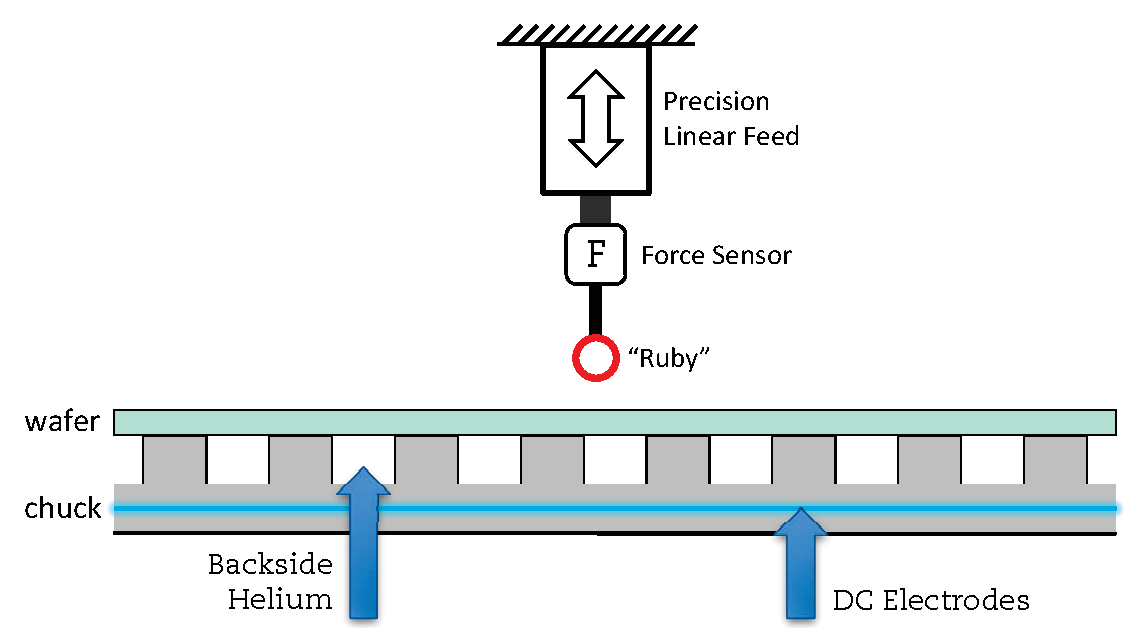
\includegraphics[width=1\linewidth]{rig/overall__sch}
\caption{测量平台总体设计示意}
\label{fig:rig-overall-sch}
\end{figure}

如图~\ref{fig:rig-overall-sch},整个测量平台由以下组件构成:

\begin{itemize}
  \item 待测静电卡盘及其配套静电电源
  \item 微力探头组件
  \item 背吹控制系统
  \item 机械结构
  \item 电控与数据采集系统
\end{itemize}

除静电卡盘与电源外,其他组件均需自行设计、搭建。


\subsection{检测流程}

一次完整的检测过程分如下步骤完成:

\begin{enumerate}
  \item 准备静电卡盘
  \begin{enumerate}
    \item 用无水乙醇擦拭静电卡盘与晶圆
    \item 将晶圆小心地放置在静电卡盘陶瓷层正中央
    \item 开启静电电源,调节电极电压至目标电压
  \end{enumerate}
  
  \item 准备测量平台
  \begin{enumerate}
    \item 降下微力探头,使其轻轻接触晶圆
    \item 确认背吹控制系统中调压装置均处于零位
  \end{enumerate}
  
  \item 检测
  \begin{enumerate}
    \item 开始自动记录微力探头受力、背吹入口气压两变量
    \item 背吹气压接通并缓慢、均匀地上升
    \item 当微力探头受力即将达到其满量程时,自动切断背吹气压,检测停止
  \end{enumerate}
  
  \item 后续处理
  \begin{enumerate}
    \item 导出采集到的数据
    \item 微力探头复位上升
    \item 切断静电电源,短接两电极引线,消除部分残余电荷
    \item 小心将晶圆取下
  \end{enumerate}
\end{enumerate}



\section{微力探头组件设计}\label{sec:rig-probe}

图~\ref{fig:rig-sch}中,卡盘上方的组件即为微力探头组件微力探头组件,其在\ref{principle-gap-ruby}一节中提到的微力传感器和红宝石探头的基础上,增设精密直线进给机构:固定端连接在框架上,移动端与力传感器的固定端相连,用于驱动探头沿z方向移动,以实现“轻轻接触晶圆”这一动作。


\subsection{微力传感器选型}\label{sec:rig-probe-sensor}

微力传感器是探头组件中的核心元件,因此优先选型。考虑到其在测量系统中的作用,主要关心以下参数:

\begin{enumerate}
  \item \textbf{量程}:
    无论在轻触阶段还是在脱附检测阶段,探头均不应向晶圆施加过大的力。粗估静电力处于$\SI{10}{\newton}$至$\SI{200}{\newton}$之间,探头施加的力应低于其$1 ~\%$,即微力传感器应能准确测量 大致在$\SI{0.1}{\newton}$至$\SI{2}{\newton}$范围内的单轴压缩力。
  \item \textbf{分辨力}:
    微力传感器需能检测到微小的受力变化,根据上述关于量程的讨论,应能至少分辨出$\SI{1}{\milli\newton}$的力增量。不同的传感器可能对分辨力的标称方法不同,应结合其输出信号特点,判定其是否满足要求。
  \item \textbf{刚度}:
    微力传感器的敏感端存在一位移,一般服从胡克定律,与受力成比例关系。\ref{principle-gap}一节中讨论了晶圆与卡盘间气隙可能对静电力产生的影响。若传感器刚度较高,则可更好地控制气隙大小,并在气隙明显扩大之前检测出脱附;但另一方面,高刚度使轻触晶圆更难实现(见\ref{rig-probe-feeding}节\ \eqref{eq:rig-probe-feeding-vel}式)。因此该参数并无明确要求,仅做为选型时的参考。
  \item \textbf{过载能力}:
    考虑到在安装、调试过程中,以及硅晶圆突然完全脱附时,探头均可能瞬间受到较大的力的作用;若微力传感器承受过载能力较好,则可避免其意外受损。
\end{enumerate}

初步筛选市面上各种微力传感器得到表~\ref{tab:rig-probe-sensor}。若考虑量程、精度、分辨力,1050V1较差;若考虑刚度,LSB200较差;若考虑过载性能,FT-S10000较差。由上文讨论,量程、分辨力是最重要的性能指标,而刚度因素较为次要,且即使是刚度最低的LSB200,其值也已达到$\SI[per-mode=symbol]{1}{\milli\newton\per\micro\meter}$,因此选择LSB200型应变式微力传感器。

% generated using http://www.tablesgenerator.com/latex_tables
\begin{table}[htbp]
\begin{minipage}{1\linewidth}
\centering
\caption{微力传感器选型表}
\label{tab:rig-probe-sensor}
\begin{tabular}{@{}lllccc@{}}
\toprule[1.5pt]
生产商 &  &  & Futek & Dytran & FemtoTech \\
型号 &  &  & LSB200 & 1050V1 & FT-S10000 \\
\midrule[1pt]
原理 &  &  & 应变式 & 压电式 & MEMS \\
输出信号 & 类型 &  & 电阻电桥 & 电压 & 电压 \\
 & 单位 &  & $\si[per-mode=symbol]{\milli\volt\per\volt}$ & V & V \\
灵敏度 & 满量程 & 输出 & 0.5 & 5 & 2 \\
 & 单位受力 & 输出/$\si{\newton}$ & 5.0E+00 & 1.1E-01 & 2.0E+02 \\
分辨力 &  & $\si{\micro\newton}$ & --\footnote{未标称,下同} & 600 & 0.5 \\
刚度 &  & $\si[per-mode=symbol]{\newton\per\micro\meter}$ & 0.001 & 1996.45 & -- \\
\midrule[1pt]
满量程 & 拉(+) & $\si{\newton}$ & 0.1 & 44.48 & 0.01 \\
 & 压(-) & $\si{\newton}$ & 0.1 & 44.48 & 0.01 \\
最大载荷 & 拉(+) & $\si{\newton}$ & 1 & 889.64 & 0.03 \\
 & 压(-) & $\si{\newton}$ & 1 & 889.64 & 0.03 \\
\midrule[1pt]
线性度 &  & \% FS & 0.1 & 1 & \multirow{2}{*}{--} \\
 &  & $\si{\newton}$ & 2.00E-04 & 8.90E-01 &  \\
滞回 &  & \% FS & 0.1 & \multirow{2}{*}{--} & \multirow{2}{*}{--} \\
 &  & $\si{\newton}$ & 2.00E-04 &  &  \\
重复精度 &  & \% FS & 0.05 & \multirow{2}{*}{--} & \multirow{2}{*}{--} \\
 &  & $\si{\newton}$ & 1.00E-04 &  &  \\
\bottomrule[1.5pt]
\end{tabular}
\end{minipage}
\end{table}


\subsection{进给机构选型}\label{sec:rig-probe-feeding}

进给机构的主要作用为完成“轻触晶圆”动作,其移动组件可为推杆或直线滑移台(优先推杆),驱动方式可为手动或电动(优先电动)。对于手动进给机构,只需考虑其最小步长(受静摩擦等因素限制),因此下面主要讨论电动进给机构的选型。主要关心以下参数:

\begin{enumerate}
  \item \textbf{低速性能}:
    由于当探头接触到晶圆时,接触力会突增,为了限制接触力,需要控制探头以较低速度接近晶圆,直至微力传感器读数出现明显变化,即命令进给机构停止运动。这要求进给机构能够在低速下平稳运行,即低速速度波动较小,或爬行现象不明显。参考运动速度可按\eqref{eq:rig-probe-feeding-vel}计算:
    \begin{equation}
    \label{eq:rig-probe-feeding-vel}
    v_{\mathrm{ref}} = \frac{ F_{\mathrm{thres}} }
                            { k_{\mathrm{sensor}} \cdot t_{\mathrm{delay}} }
    \end{equation}
    其中:
    \begin{itemize}
      \item $F_{\mathrm{thres}}$  : 探头接触晶圆时最大允许施加的力
      \item $k_{\mathrm{sensor}}$ : 微力传感器刚度
      \item $t_{\mathrm{delay}}$  :  从探头受力跳变到进给机构停止运动的总时滞(包括机械惯性、信号传输延迟等)
    \end{itemize}
    代入LSB200相关数据(
    $F_{\mathrm{thres}} = \SI{1}{\milli\newton}$,
    $k_{\mathrm{sensor}} = \SI[per-mode=symbol]{0.001}{\newton\per\micro\meter}$
    ),在$t_{\mathrm{delay}} = \SI{0.01}{\second}$时计算参考速度为$\SI[per-mode=symbol]{100}{\micro\meter\per\second}$。
  \item \textbf{总行程}:
    小型精密电动进给机构行程较低,可采用粗精二级调节的方法:先用手动或电动方式粗调整个微力探头组件,将其固定在接近晶圆的位置上,再驱动精密进给机构完成轻触动作。为了方便粗调,希望总行程至少为$\SI{5}{\milli\meter}$。
  \item \textbf{背隙/回差/抖动}:
    完成轻触晶圆动作后,进给机构需保持原位不动(锁定),因此对于能够自锁的机构,不应有回差影响;对于不能自锁的机构,需确认其抖动在合理范围内。
\end{enumerate}

由于候选型号较多,完整的选型表参见附录B。 %TODO:xref appendix
最终选定的电动进给机构为LAC10A-T4精密电动推杆,其原理为步进电机驱动滚珠丝杠,有效行程$\SI{10}{\milli\meter}$,重复定位精度$\pm\SI{1.5}{\micro\meter}$。



\section{背吹控制系统设计}\label{sec:rig-pressure}

%TODO:update pressure schematic
\begin{figure}[tbh]
\centering
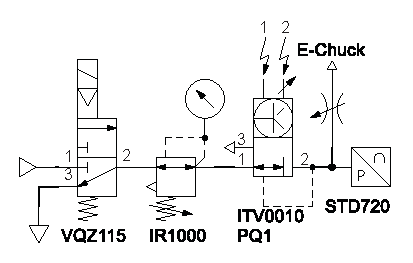
\includegraphics[width=0.618\linewidth]{rig/pressure__sch__full}
\caption{整体气路图}
\label{fig:rig-pressure-sch-full}
\end{figure}



\section{机械结构设计}\label{sec:rig-model}

\begin{figure}[p]
\centering
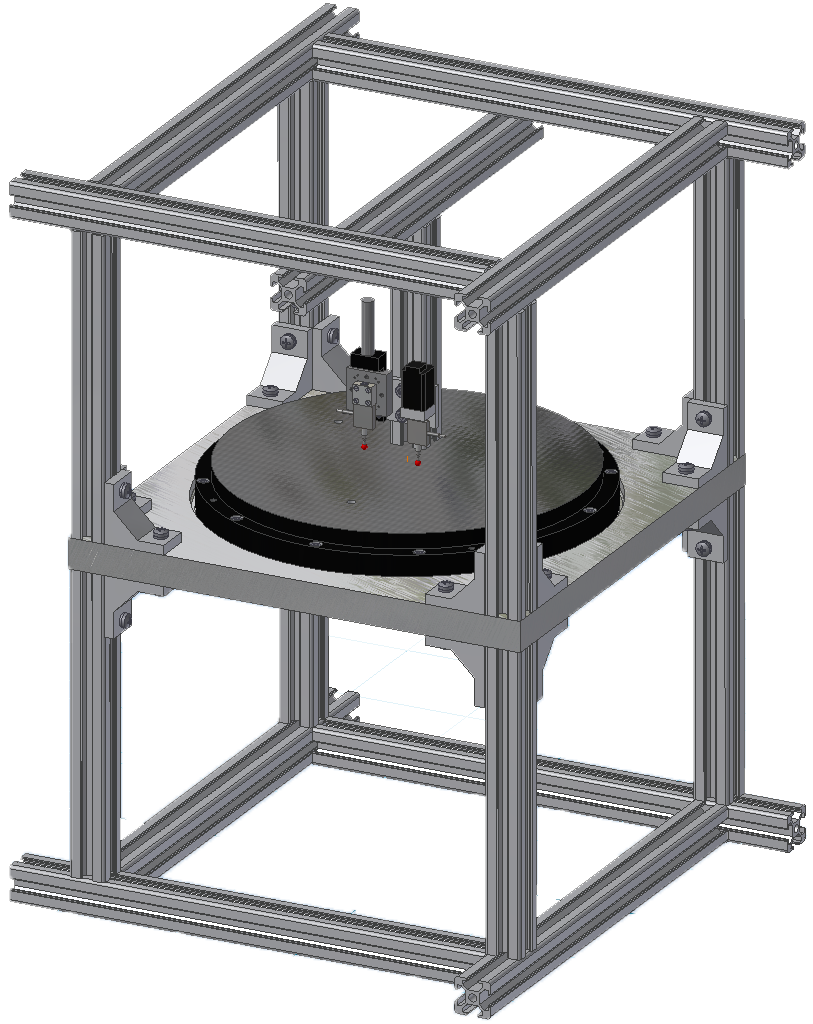
\includegraphics[width=1\textwidth]{rig/model__all__iso.png}
\caption{试验台整体数字模型}
\label{fig:rig-model-all-iso}
\end{figure}

\begin{figure}[tbhp]
\centering
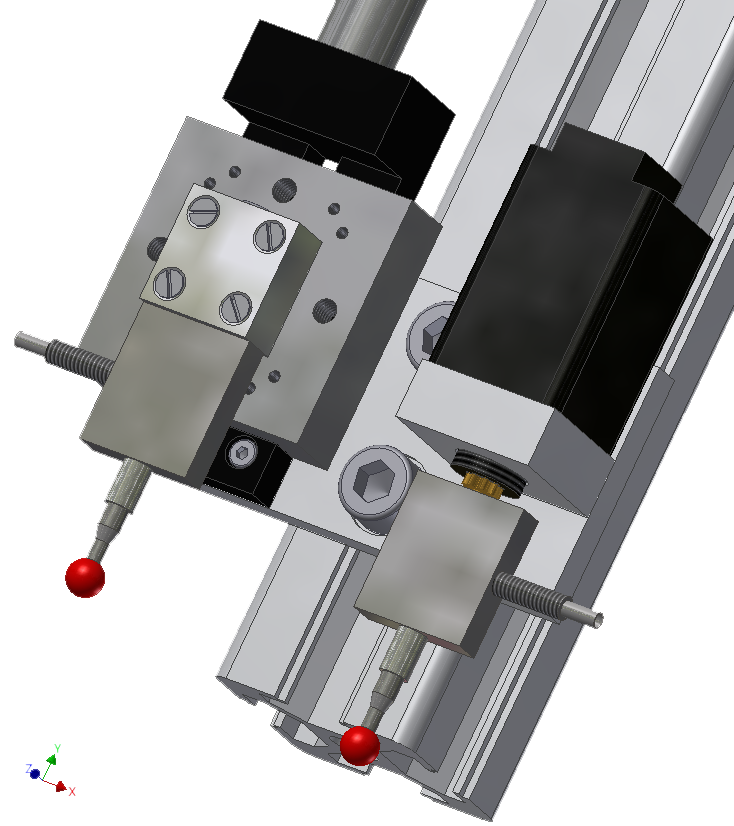
\includegraphics[height=0.45\textheight]{rig/model__probe.png}
\caption{探头组件数字模型}
\label{fig:rig-model-probe}
\end{figure}



\section{电控与数据采集系统设计}